\section{Participation notes 6}
Participant: Student

\begin{itemize}
    \item \textbf*{Have them read the code-example} - Participant did not have any problem reading the code.
    \item \textbf*{Have them draw the structure} - The participant focused on the output of the code. Visualized the "cout" as speach bubles and the code base as a blueprint.
    \item \textbf*{Have them submit the git URL} - URL submission went without any problem and camera controlls seemed to be intuitive.
    \item \textbf*{Have them get the main() implementation} - Fetching implementation of main function worked without any problem. Participant also used the code on paper and visualization for navigation of calls. Other functions implementation wasn't intuitive to fetch.
    \item \textbf*{Participant visualization} \includepdf[pages={5}]{inc/generalAppendix/userStudies/participantsVisualization.pdf}
\end{itemize}